\documentclass{article}
\usepackage{graphicx} % Required for inserting images
\usepackage[colorlinks=true, linkcolor=blue, urlcolor=blue, framecolor=blue]{hyperref} % Customize link and box colors
\usepackage{float}
\usepackage{amsmath}

% Adjust page margins
\usepackage[margin=1in]{geometry} % Adjust the margin size as needed

\title{Machine Learning Report on Energy Consumption of Fischertechnik Sorting Line}
\author{Aaditya Neupane}
\date{May 2025}

\begin{document}

\maketitle

\section{Introduction}
\begin{itemize}
    \item This report shows Data collection, Preparation, Feature Extraction and Selection, Feature Reduction, and approaches used to train ml models on data collected from the Fischertechnik Sorting Line.

\end{itemize}


\section{Data Collection}
\begin{itemize}
    \item Energy consumption data on following objects were collected from Sorting Line using an arduino. Each time an object is passed through the sorting line it recorded the energy data into a CSV file.
    \begin{figure}[h]
        \centering
        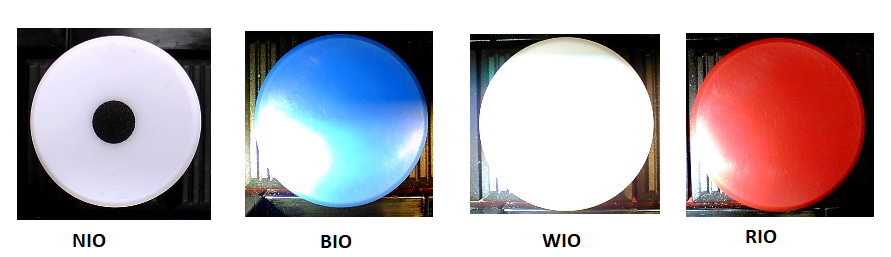
\includegraphics[width=1\linewidth]{objects.png}
        \caption{Objects}
        \label{fig:labels}
    \end{figure}
    \item Data was collected at different frequencies: 100hz, 400hz, 800hz
    \item Data for each objects were recorded 1000 times; creating 4000 total data for each frequency
    \item Initial features on the collected data: \\
    Datum, Uhrzeit, I\_In, V\_In,  P\_In(W), I\_Out(A), V\_Out(V), P\_Out(W), Temp(°C), Energie\_In(Wh), Energie\_Out(Wh)
\end{itemize}

\section{Data Preperation}
\begin{itemize}
    \item For each frequency, all the individual csv files for all objects were merged.
    \item While merging, new column was added to indicate rows their particular object-labels
    \\
    (target column : "color")
    \item Following Unnecessary and Derived columns were dropped: 'Datum', 'P\_In(W)','P\_Out(W)', \\ 'Energie\_In(Wh)','Energie\_Out(Wh)'
    \item Then the dataframe was divided into train and test and saved as csv files on different train:test ratios:- 
    \\
    20:80, 50:50, 80:20
\end{itemize}


\section{Feature Extraction and Selection}
\begin{itemize}
    \item Features were extracted using 2 methods:
    \begin{itemize}
        \item Tsfresh
        \item Wavelet Transformation
    \end{itemize}

    \item For Wavelet Transformation, "energy", "entropy", "variance" features were extracted at Decomposition levels of 2,3, and 4 . Then it was used to train and test the models
    \item Tsfresh was used to extract and select features. Then, the selected features were used to train and test the models.
    
\end{itemize}


\section{ML models and Result}


\begin{itemize}
    \item Following models were trained:
    \begin{itemize}
        \item XGBoost
        \item RandomForest
    \end{itemize}
    \item Results using Tsfresh :

        \begin{figure}[h]
            \centering
            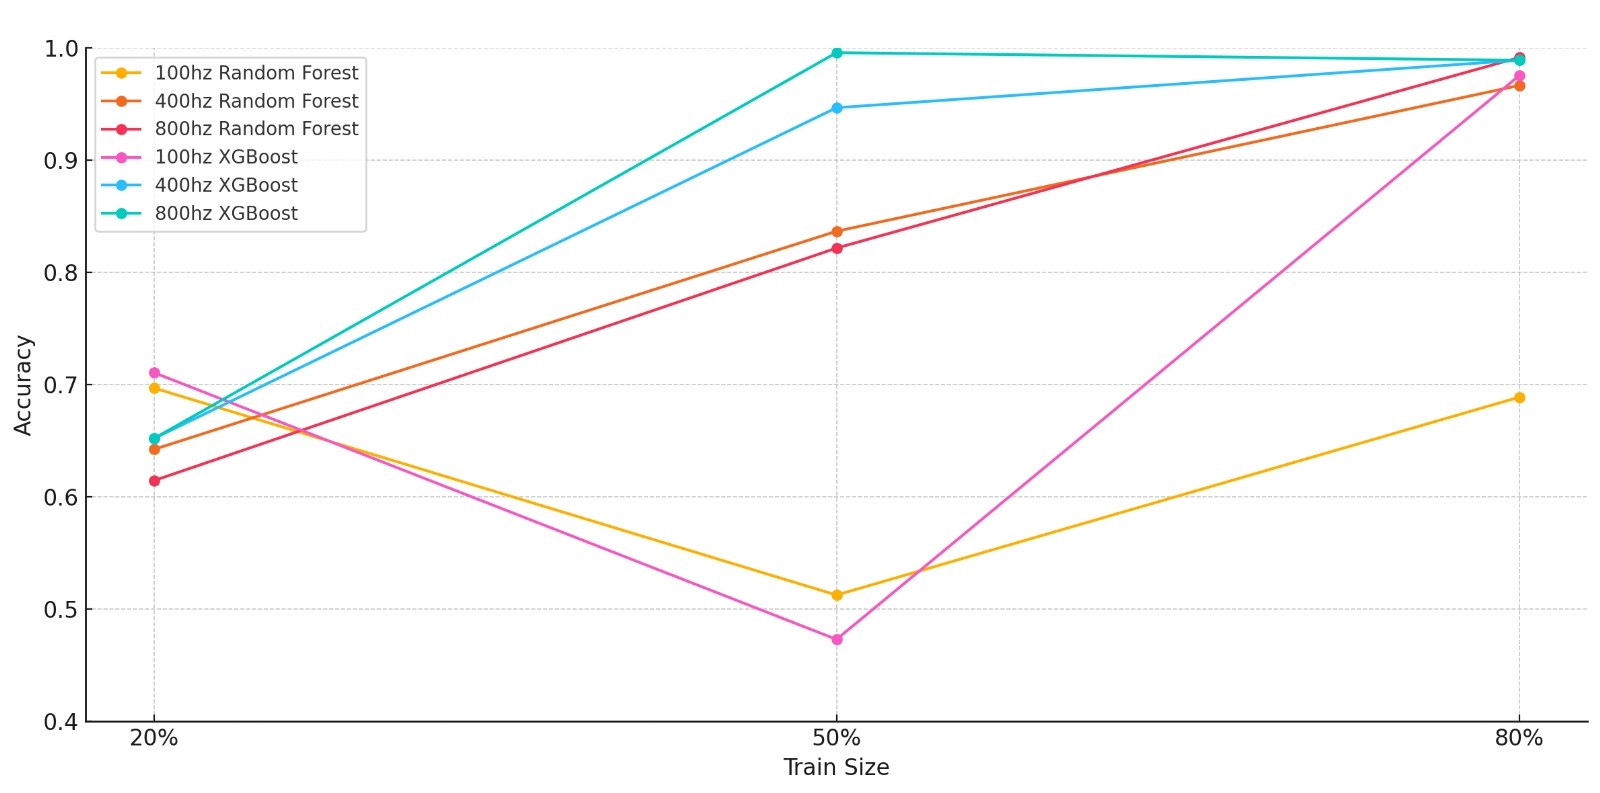
\includegraphics[width=1\linewidth]{tsfresh-img.jpg}
            \caption{Tsfresh: Model accuracy vs Training size}
            \label{fig:enter-label}
        \end{figure}
    \clearpage
    \vspace*{-1cm}
    \item Results using Wavelet Transformation:
        \begin{itemize}
            \item With 20\% Train Data
                \begin{figure}[h]
                    \centering
                    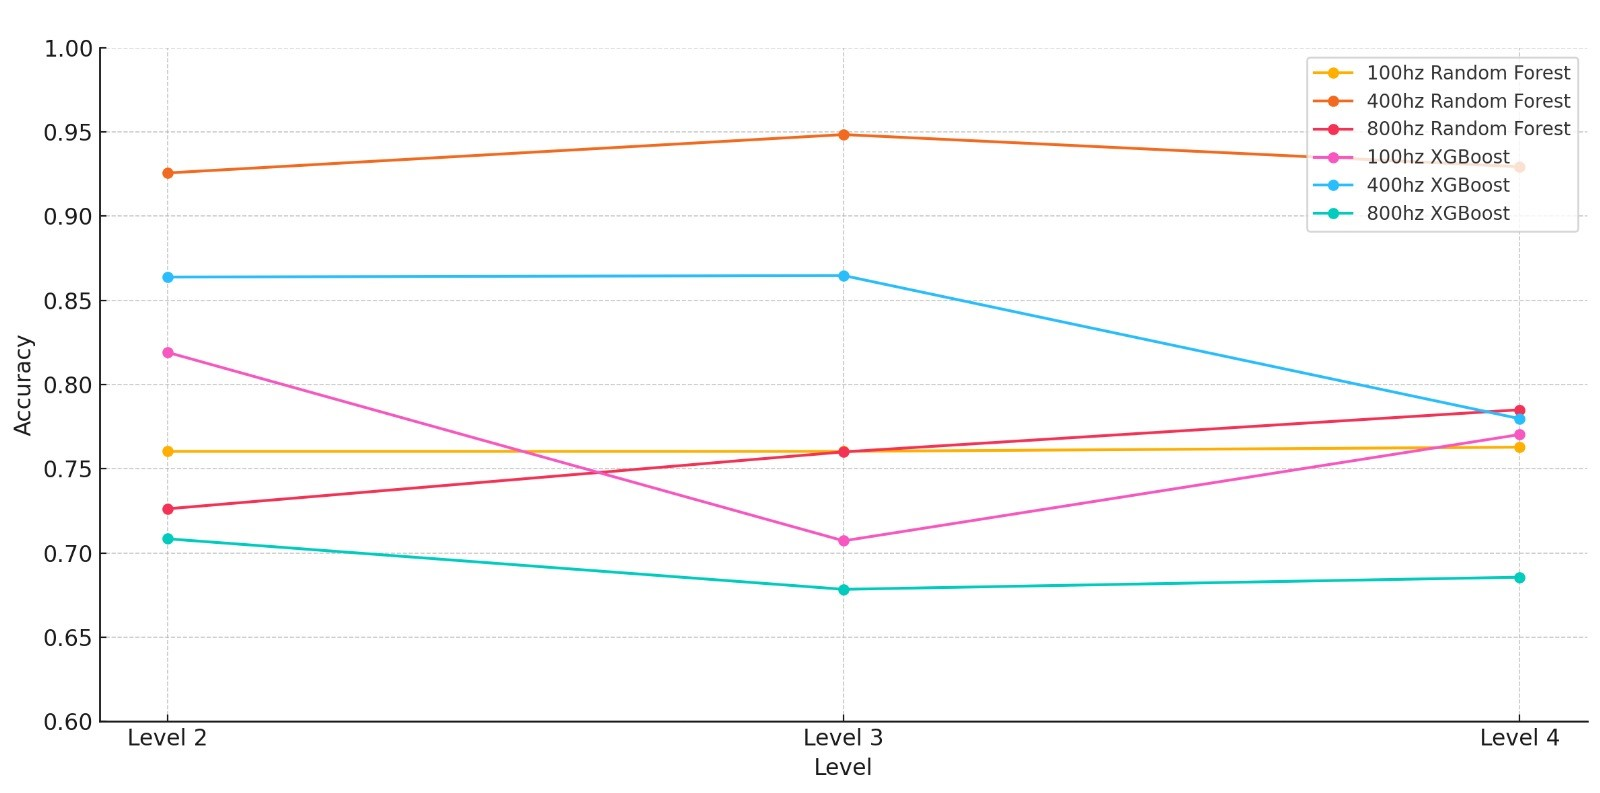
\includegraphics[width=1\linewidth]{wavelet_20_percent.jpg}
                    \caption{Wavelet Transformation: Model accuracy vs Decomposition Level}
                    \label{fig:Wavelet_transformation_20}
                \end{figure}
            \vspace{0.8cm}
            \item With 50\% Train Data
                \begin{figure}[H]
                    \centering
                    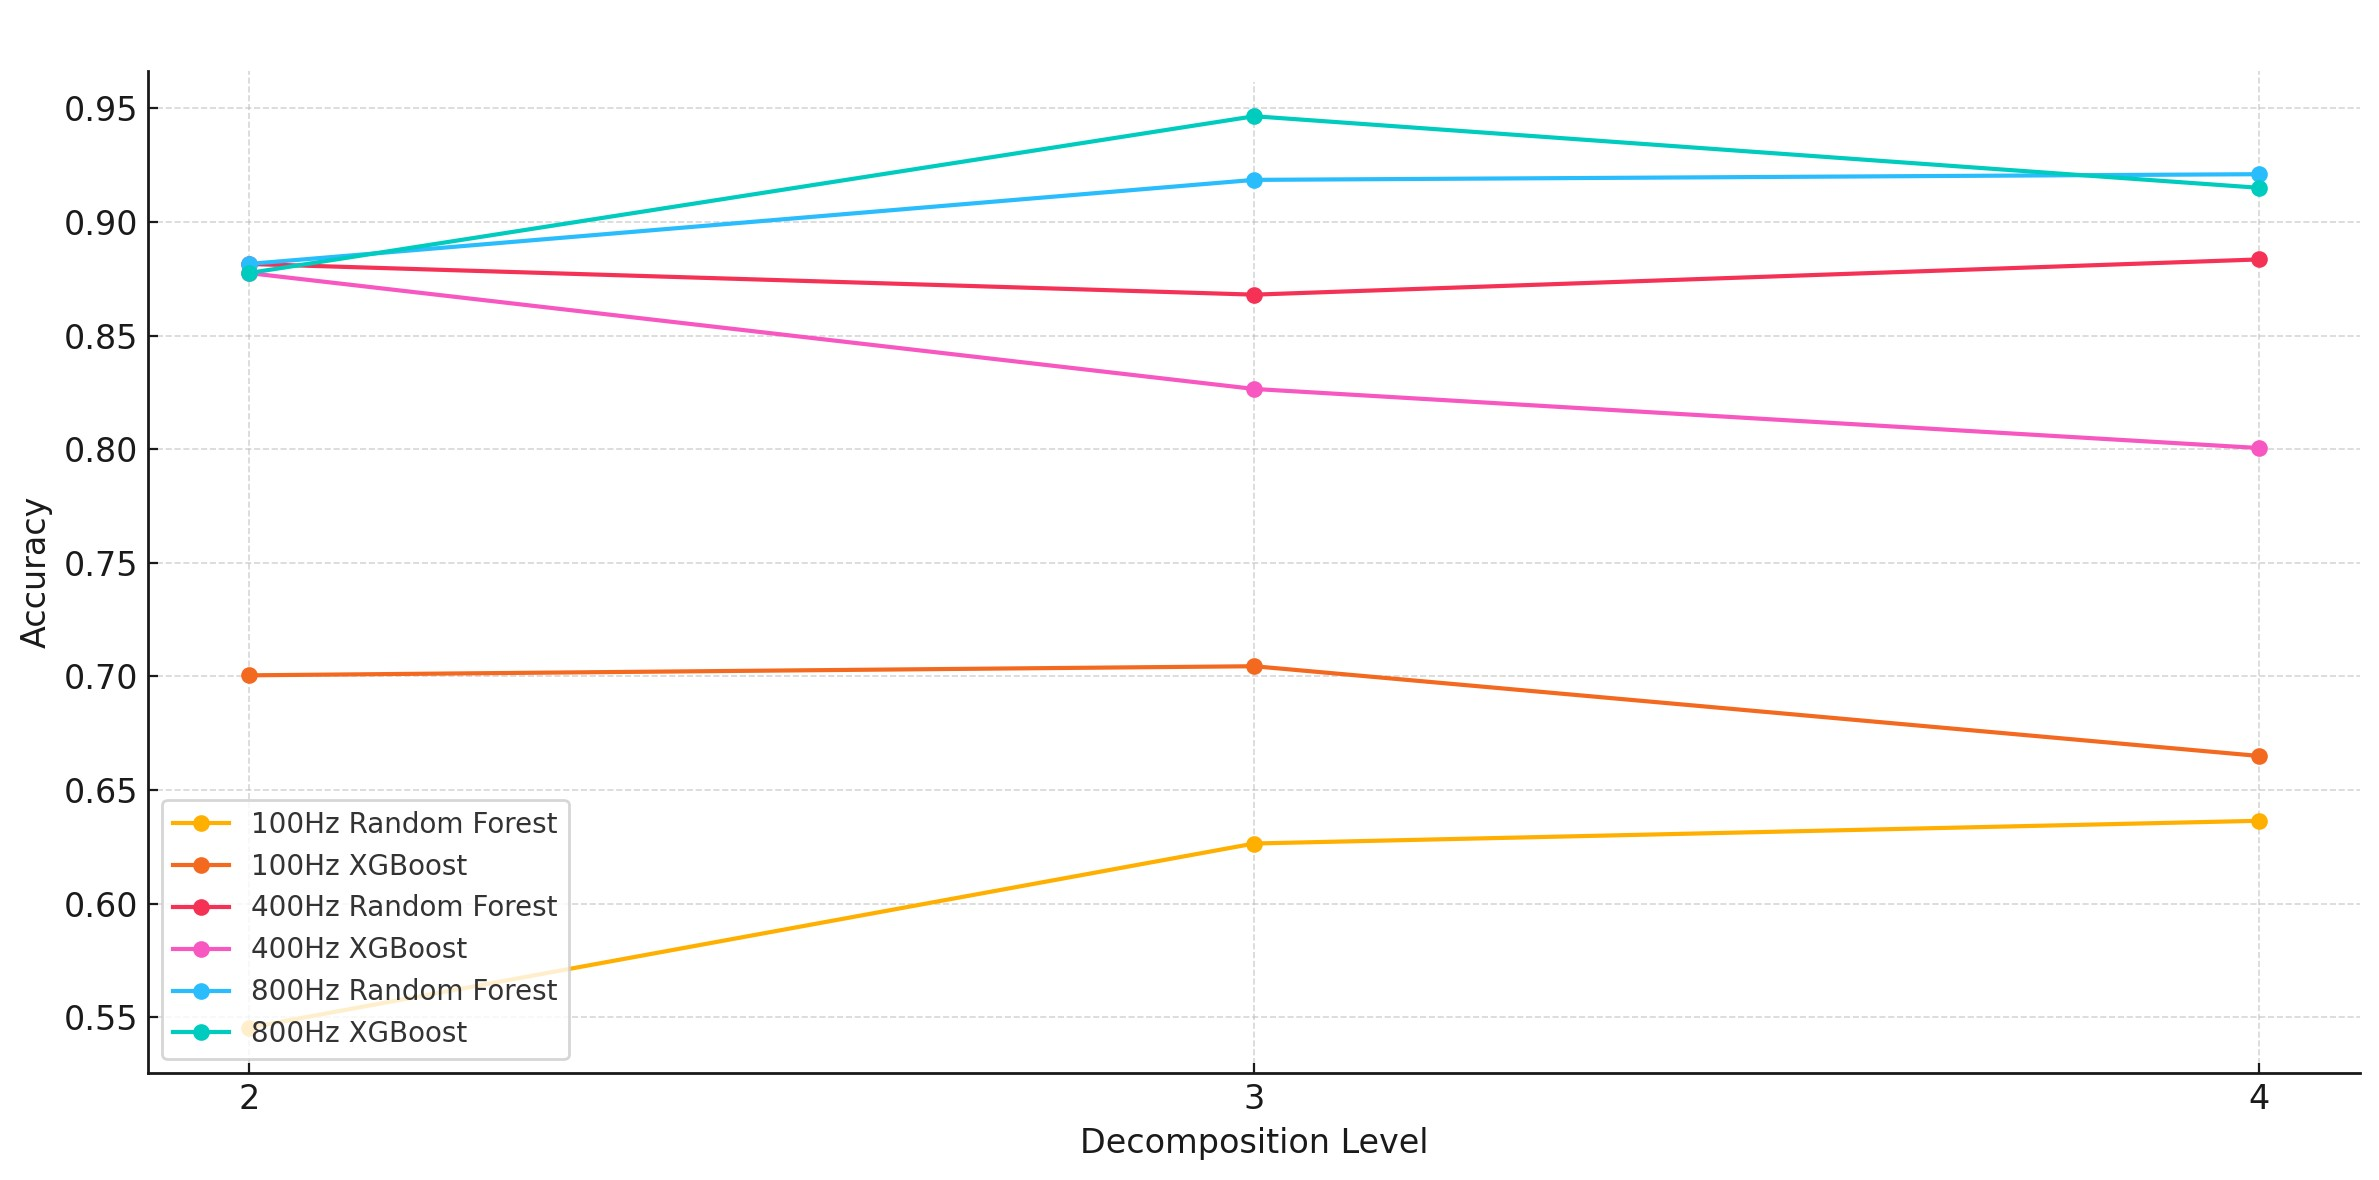
\includegraphics[width=1\linewidth]{wavelet_50_percent.jpg}
                    \caption{Wavelet Transformation: Model accuracy vs Decomposition Level}
                    \label{fig:Wavelet_transformation_50}
                \end{figure}
            \vspace{0.8cm}  
            \item With 80\% Train Data
                \begin{figure}[h]
                    \centering
                    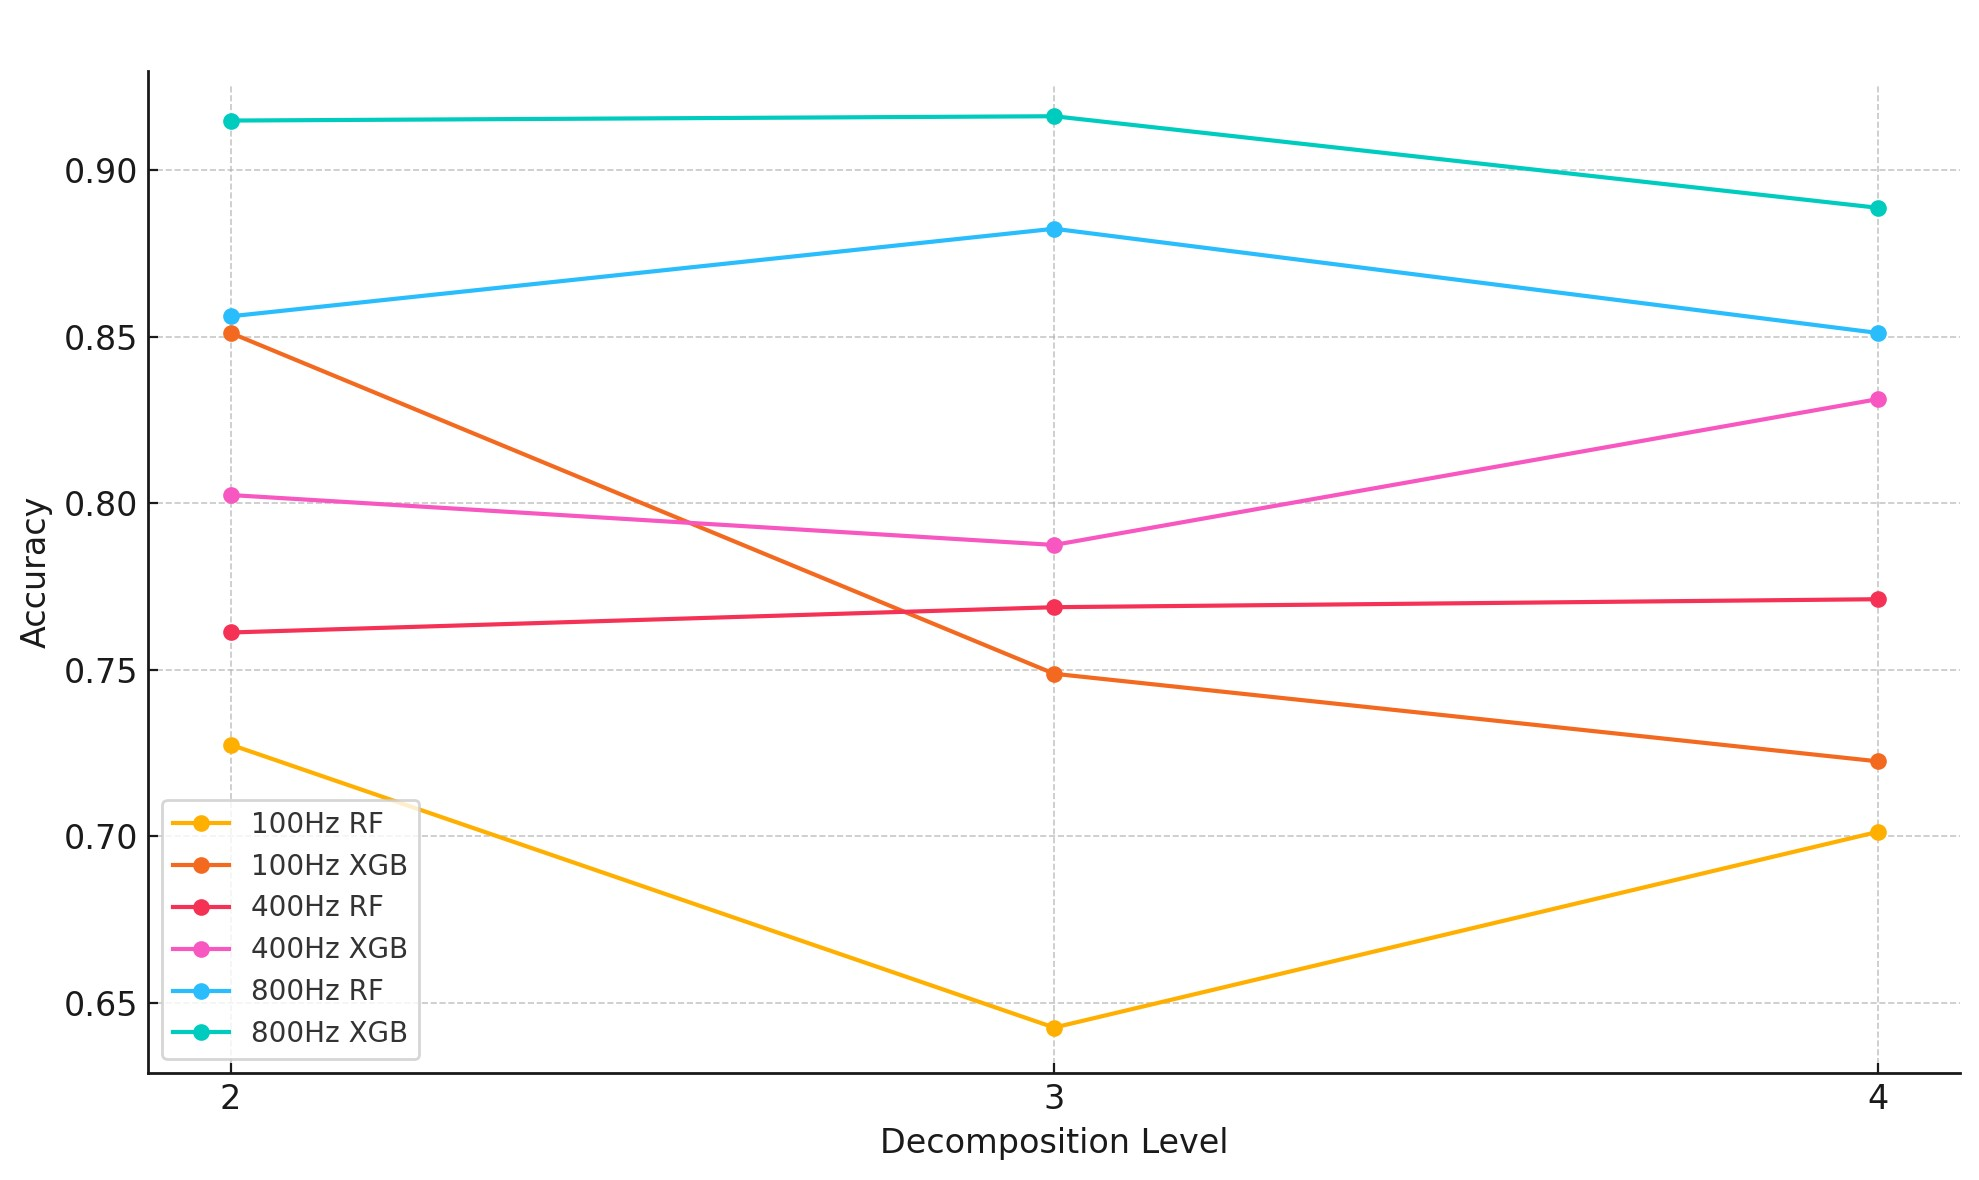
\includegraphics[width=1\linewidth]{wavelet_80_percent.jpg}
                    \caption{Wavelet Transformation: Model accuracy vs Decomposition Level}
                    \label{fig:Wavelet_transformation_80}
                \end{figure}
        \end{itemize}
    \item Best models with Tsfresh:
        \begin{itemize}
            \item 100hz : XGBoost with 80\% train split 
            \\
            Accuracy: 0.9750
            \\
            Precision: 0.9766
            \[
            \begin{bmatrix}
            198 & 0 & 0 & 2 \\
            0 & 188 & 0 & 12 \\
            0 & 1 & 195 & 4 \\
            0 & 1 & 0 & 199
            \end{bmatrix}
            \]

            \item 400hz : XGBoost with 80\% train split
            \\
            Accuracy: 0.9888
            \\
            Precision: 0.9889
            \[
            \begin{bmatrix}
            199 & 0   & 1   & 0 \\
            0   & 197 & 3   & 0 \\
            1   & 1   & 198 & 0 \\
            0   & 1   & 2   & 197
            \end{bmatrix}
            \]
            

            \item 800hz : XGBoost with 50\% train split
            \\
            Accuracy: 0.9955
            \\
            Precision: 0.9955
            \\
            \[
            \begin{bmatrix}
            499 & 0   & 1   & 0 \\
            0   & 495 & 0   & 5 \\
            2   & 0   & 497 & 1 \\
            0   & 0   & 0   & 500
            \end{bmatrix}
            \]


        \end{itemize}
        \item Best models with Wavelet Transformation:
        \begin{itemize}
            \item 100hz : XGBoost with Decomposition level 2 on 80\% train split
            \\
            Accuracy: 0.8512
            \\
            Precision: 0.8614
            \[
            \begin{bmatrix}
            188 & 0   & 11  & 1 \\
            0   & 166 & 9   & 25 \\
            0   & 67  & 133 & 0 \\
            0   & 6   & 0   & 194
            \end{bmatrix}
            \]

            
            \item 400hz : RandomForest with Decomposition level 3 on 20\% train split

            Accuracy  0.9484
            \\
            Precision 0.9487
            \\
            \[
            \begin{bmatrix}
            776 & 0   & 24  & 0 \\
            0   & 743 & 40  & 17 \\
            14  & 28  & 750 & 8 \\
            0   & 34  & 0   & 766
            \end{bmatrix}
            \]


            \item 800hz : XGBoost with Decomposition level 3 on 50\% train split
                
            Accuracy: 0.9465
            \\
            Precision: 0.9483
            \\
            \[
            \begin{bmatrix}
            499 & 0   & 0   & 1 \\
            0   & 470 & 11  & 19 \\
            19  & 20  & 428 & 33 \\
            0   & 4   & 0   & 496
            \end{bmatrix}
            \]
            
        \end{itemize}
    
\end{itemize}
\section{Feature Reduction}
\begin{itemize}
    \item Since, 800hz XGBoost 50\% train split with Tsfresh trained the best model, same extracted features was used for feature reduction.
    \item Features were selected based on the importance of features.
    \item Before feature reduction (2122 features)
    \begin{itemize}
            \\
            Accuracy: 0.9955
            \\
            Precision: 0.9955
            \\
            \[
            \begin{bmatrix}
            499 & 0   & 1   & 0 \\
            0   & 495 & 0   & 5 \\
            2   & 0   & 497 & 1 \\
            0   & 0   & 0   & 500
            \end{bmatrix}
            \]
    \end{itemize}
    

    \item Reduction to 187 features
        \begin{itemize}
            Accuracy: 0.9955
            \\
            Precision: 0.9955
            \\
            \[
            \begin{bmatrix}
            499 & 0   & 1   & 0 \\
            0   & 496 & 0   & 4 \\
            2   & 1   & 496 & 1 \\
            0   & 0   & 0   & 500
            \end{bmatrix}
            \]
            
        \end{itemize}
        \clearpage
    

    
    \item Reduction to 50 Features
    \begin{itemize}
 
        Accuracy: 0.9930
        \\
        Precision: 0.9931
        \\
        \[
        \begin{bmatrix}
        499 & 0   & 1   & 0 \\
        1   & 490 & 2   & 7 \\
        2   & 0   & 497 & 1 \\
        0   & 0   & 0   & 500
        \end{bmatrix}
        \]
    \end{itemize}
    

    \item Reduction to a single Feature
    \begin{itemize}
 
        Accuracy: 0.9395
        \\
        Precision: 0.9403
        \\
        \[
        \begin{bmatrix}
        498 & 0   & 1   & 1 \\
        0   & 421 & 61  & 18 \\
        9   & 11  & 479 & 1 \\
        0   & 19  & 0   & 481
        \end{bmatrix}
        \]

    \end{itemize}
    \\
    \vspace{1cm}
    \\
    \begin{figure}[h]
        \centering
        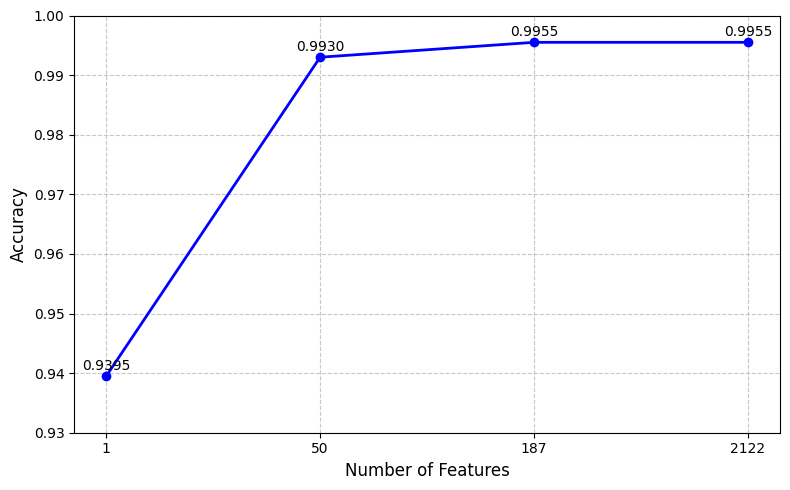
\includegraphics[width=1\linewidth]{feature_reduction.jpg}
        \caption{Impact of Feature Reduction}
        \label{fig:feature_reduction_impact}
    \end{figure}

\end{itemize}
\end{document}

